% ============================================================
% PART 3: Section 4 (Implementation) + Section 5 (Simulation & Testing)
% ============================================================

% ---- SECTION 4 ----
\section{Implementation}

\subsection{Vivado Block Design and IP Packaging}

The hardware implementation was carried out in Vivado 2024.2. The AES-128 core was first packaged as a custom IP using the \textit{Package IP} wizard, creating a \texttt{component.xml} descriptor that registers the AXI4-Lite interface, clock, and reset ports for Vivado's IP Integrator.

The block design (Figure~\ref{fig:block_design}) was constructed by:
\begin{enumerate}[leftmargin=*]
    \item Instantiating a MicroBlaze soft processor with 128 KB local memory.
    \item Running \textit{Run Block Automation} to auto-add the Processor System Reset, MDM debug module, and Clocking Wizard (100 MHz).
    \item Adding the AXI BRAM Controller IP twice for independent Input (0xC0000000) and Output (0xC2000000) BRAMs.
    \item Connecting a 4 KB Block Memory Generator to each BRAM controller.
    \item Adding the custom AES-128 AXI-Lite IP from the user IP repository.
    \item Adding AXI GPIO (3 LED outputs + 2 button inputs) and AXI UART Lite.
    \item Running \textit{Run Connection Automation} to complete all AXI interconnect wiring.
\end{enumerate}

\subsection{Pin Assignments (XDC Constraints)}

The physical I/O pin assignments were defined in the Xilinx Design Constraints (XDC) file \texttt{nexys4ddr\_image\_crypto.xdc}:

\begin{lstlisting}[style=tclstyle, caption={Key XDC Pin Assignments for Nexys 4 DDR}]
# UART
set_property PACKAGE_PIN C4  [get_ports UART_txd]
set_property PACKAGE_PIN D4  [get_ports UART_rxd]
set_property IOSTANDARD LVCMOS33 [get_ports UART_txd]
set_property IOSTANDARD LVCMOS33 [get_ports UART_rxd]

# GPIO LEDs
set_property PACKAGE_PIN H17 [get_ports {GPIO_LEDS[0]}]  ;# LED0 (idle indicator)
set_property PACKAGE_PIN N15 [get_ports {GPIO_LEDS[1]}]  ;# LED16_R (encrypting)
set_property PACKAGE_PIN R11 [get_ports {GPIO_LEDS[2]}]  ;# LED16_G (done)

# GPIO Buttons
set_property PACKAGE_PIN N17 [get_ports {GPIO_BTNS[0]}]  ;# BTNC (trigger)
set_property PACKAGE_PIN P18 [get_ports {GPIO_BTNS[1]}]  ;# BTND
\end{lstlisting}

\subsection{Firmware Implementation (\texttt{main.c})}

The embedded C firmware implements the complete AES-128 CTR mode encryption loop. The firmware was built in Vitis 2024.2 targeting the MicroBlaze BSP (standalone domain).

\subsubsection{Cryptographic Parameters}

\begin{itemize}[leftmargin=*]
    \item \textbf{Key (128-bit):} \texttt{00 01 02 03 04 05 06 07 08 09 0A 0B 0C 0D 0E 0F}
    \item \textbf{IV / Initial Counter (128-bit):} \texttt{F0 E0 D0 C0 B0 A0 90 80 70 60 50 40 30 20 01 00}
    \item \textbf{Image Size:} 64$\times$64 pixels = 4096 bytes = 256 AES blocks
\end{itemize}

\subsubsection{LED State Machine}

The firmware uses three GPIO-controlled LEDs to visually indicate the encryption state:

\begin{figure}[H]
\centering
\begin{tikzpicture}[
    state/.style={rectangle, draw=blue!60, fill=blue!8, rounded corners, minimum width=3cm, minimum height=1.1cm, align=center, font=\small},
    arrow/.style={-{Stealth[length=7pt]}, thick, blue!60}
]
\node[state] (idle) at (0,0) {\textbf{IDLE}\\LED0 ON (white)};
\node[state, fill=red!10, draw=red!60] (enc) at (6,0) {\textbf{ENCRYPTING}\\LED16\_R ON (red)};
\node[state, fill=green!10, draw=green!60] (done) at (3,-3) {\textbf{DONE}\\LED16\_G ON (green)};

\draw[arrow] (idle) -- node[above, font=\small]{BTNC pressed} (enc);
\draw[arrow] (enc) -- node[right, font=\small]{256 blocks complete} (done);
\draw[arrow] (done) -- node[left, font=\small]{BTNC pressed again\\(restart)} (idle);
\end{tikzpicture}
\caption{Firmware LED State Machine: LED0=Idle, Red=Encrypting, Green=Done}
\label{fig:led_fsm}
\end{figure}

\subsubsection{Core Encryption Loop}

\begin{lstlisting}[style=cstyle, caption={CTR Mode Encryption Loop (from main.c)}]
/* Write key to AES IP */
AES_WriteKey(key);

for (uint32_t blk = 0; blk < 256; blk++) {
    uint32_t byte_off = blk * 16;

    /* 1. Read plaintext block from Input BRAM */
    for (int i = 0; i < 4; i++) {
        uint32_t w = Xil_In32(XPAR_AXI_BRAM_CTRL_0_BASEADDR + byte_off + i*4);
        plain[i*4+0] = (w >> 24) & 0xFF;
        plain[i*4+1] = (w >> 16) & 0xFF;
        plain[i*4+2] = (w >>  8) & 0xFF;
        plain[i*4+3] =  w        & 0xFF;
    }

    /* 2. Encrypt counter to get keystream block */
    AES_WriteDataIn(counter);
    AES_Start();
    AES_WaitDone();   /* Poll STATUS[0] until DONE=1 (12 cycles) */
    AES_ReadDataOut(ks);

    /* 3. XOR keystream with plaintext -> ciphertext */
    for (int i = 0; i < 16; i++)
        cipher[i] = plain[i] ^ ks[i];

    /* 4. Write ciphertext to Output BRAM */
    for (int i = 0; i < 4; i++) {
        uint32_t w = ((uint32_t)cipher[i*4+0] << 24) |
                     ((uint32_t)cipher[i*4+1] << 16) |
                     ((uint32_t)cipher[i*4+2] <<  8) |
                     ((uint32_t)cipher[i*4+3]);
        Xil_Out32(XPAR_AXI_BRAM_CTRL_1_BASEADDR + byte_off + i*4, w);
    }

    /* 5. Increment counter (big-endian) */
    for (int j = 15; j >= 0; j--)
        if (++counter[j] != 0x00) break;
}
\end{lstlisting}

\subsubsection{AES IP Software Driver (\texttt{aes\_ip\_driver.h})}

The driver provides inline C functions that abstract all AXI register read/write operations:

\begin{lstlisting}[style=cstyle, caption={Key AES IP Driver Functions (aes\_ip\_driver.h)}]
/* Poll STATUS register until DONE bit is set */
static inline void AES_WaitDone(void) {
    while (!(AES_READ(AES_REG_STATUS) & AES_STATUS_DONE)) { /* poll */ }
}

/* Pulse the START bit to begin encryption */
static inline void AES_Start(void) {
    AES_WRITE(AES_REG_CTRL, AES_CTRL_START);
}
\end{lstlisting}

\subsection{Vivado Project Screenshots}

\begin{figure}[H]
    \centering
    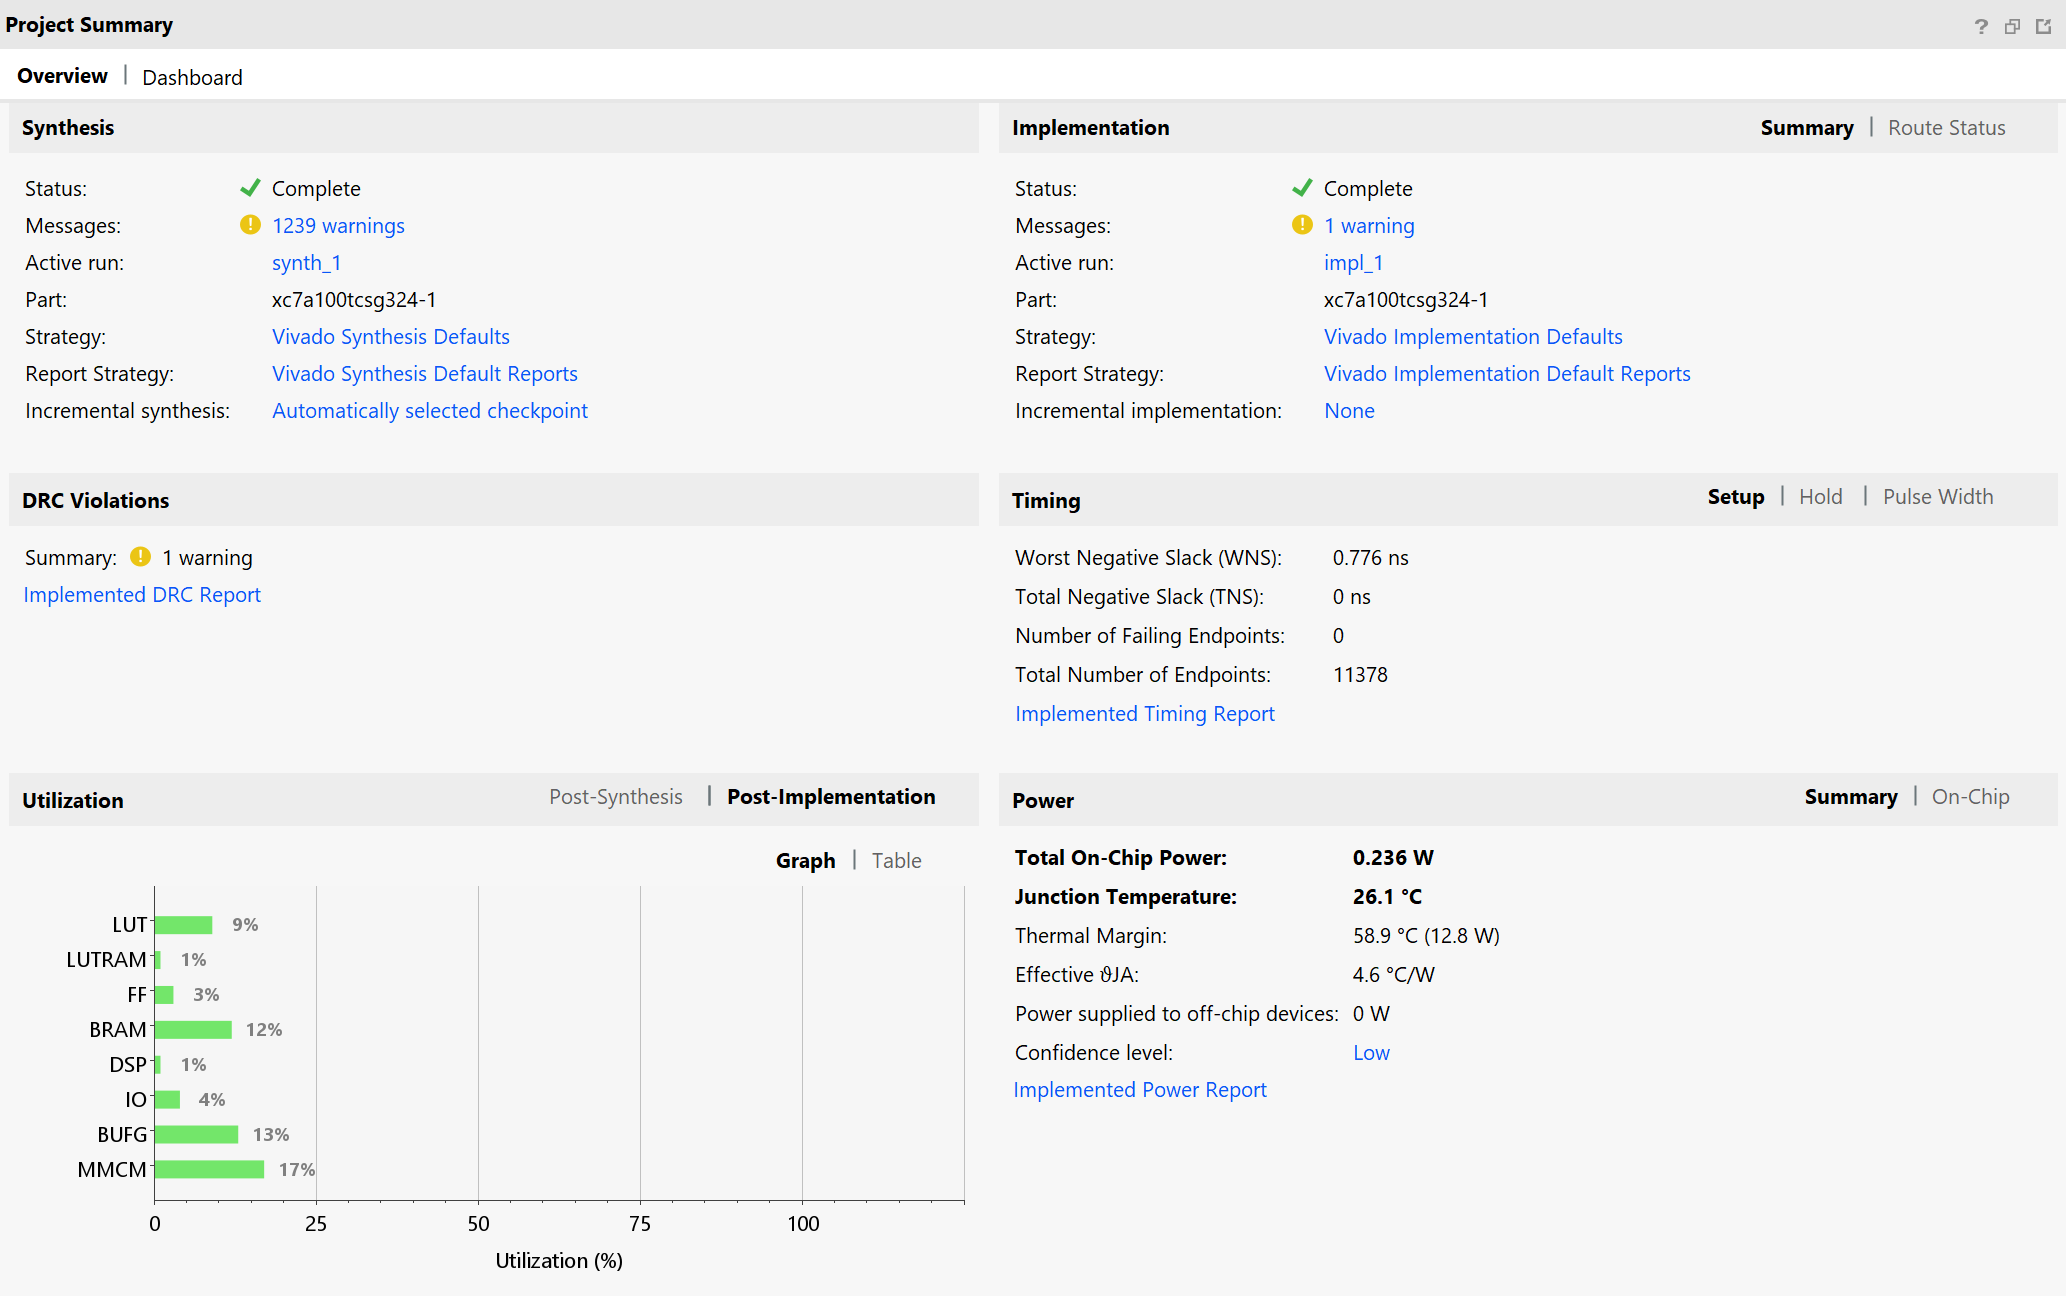
\includegraphics[width=0.9\textwidth]{project_summary.png}
    \caption{Vivado Project Summary showing design status, device, and implementation results.}
    \label{fig:proj_summary}
\end{figure}

\begin{figure}[H]
    \centering
    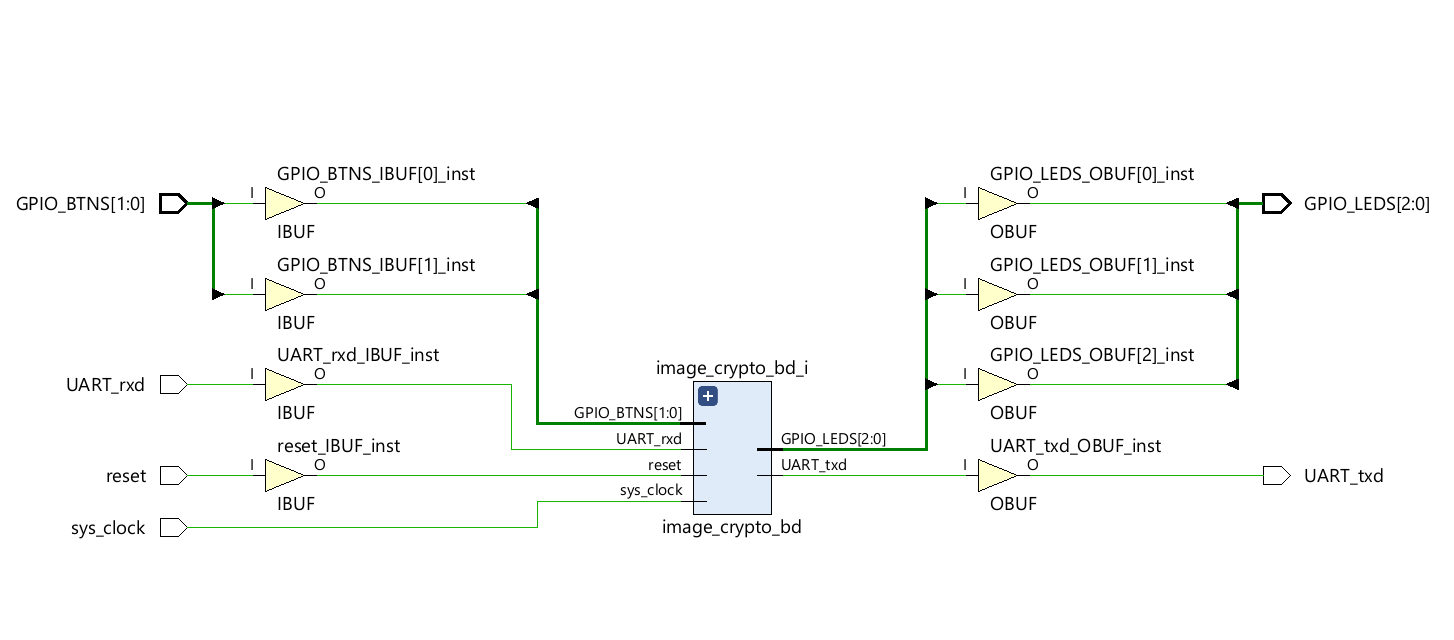
\includegraphics[width=\textwidth]{schematic.png}
    \caption{Post-Implementation Schematic View showing synthesized logic.}
    \label{fig:schematic}
\end{figure}

\begin{figure}[H]
    \centering
    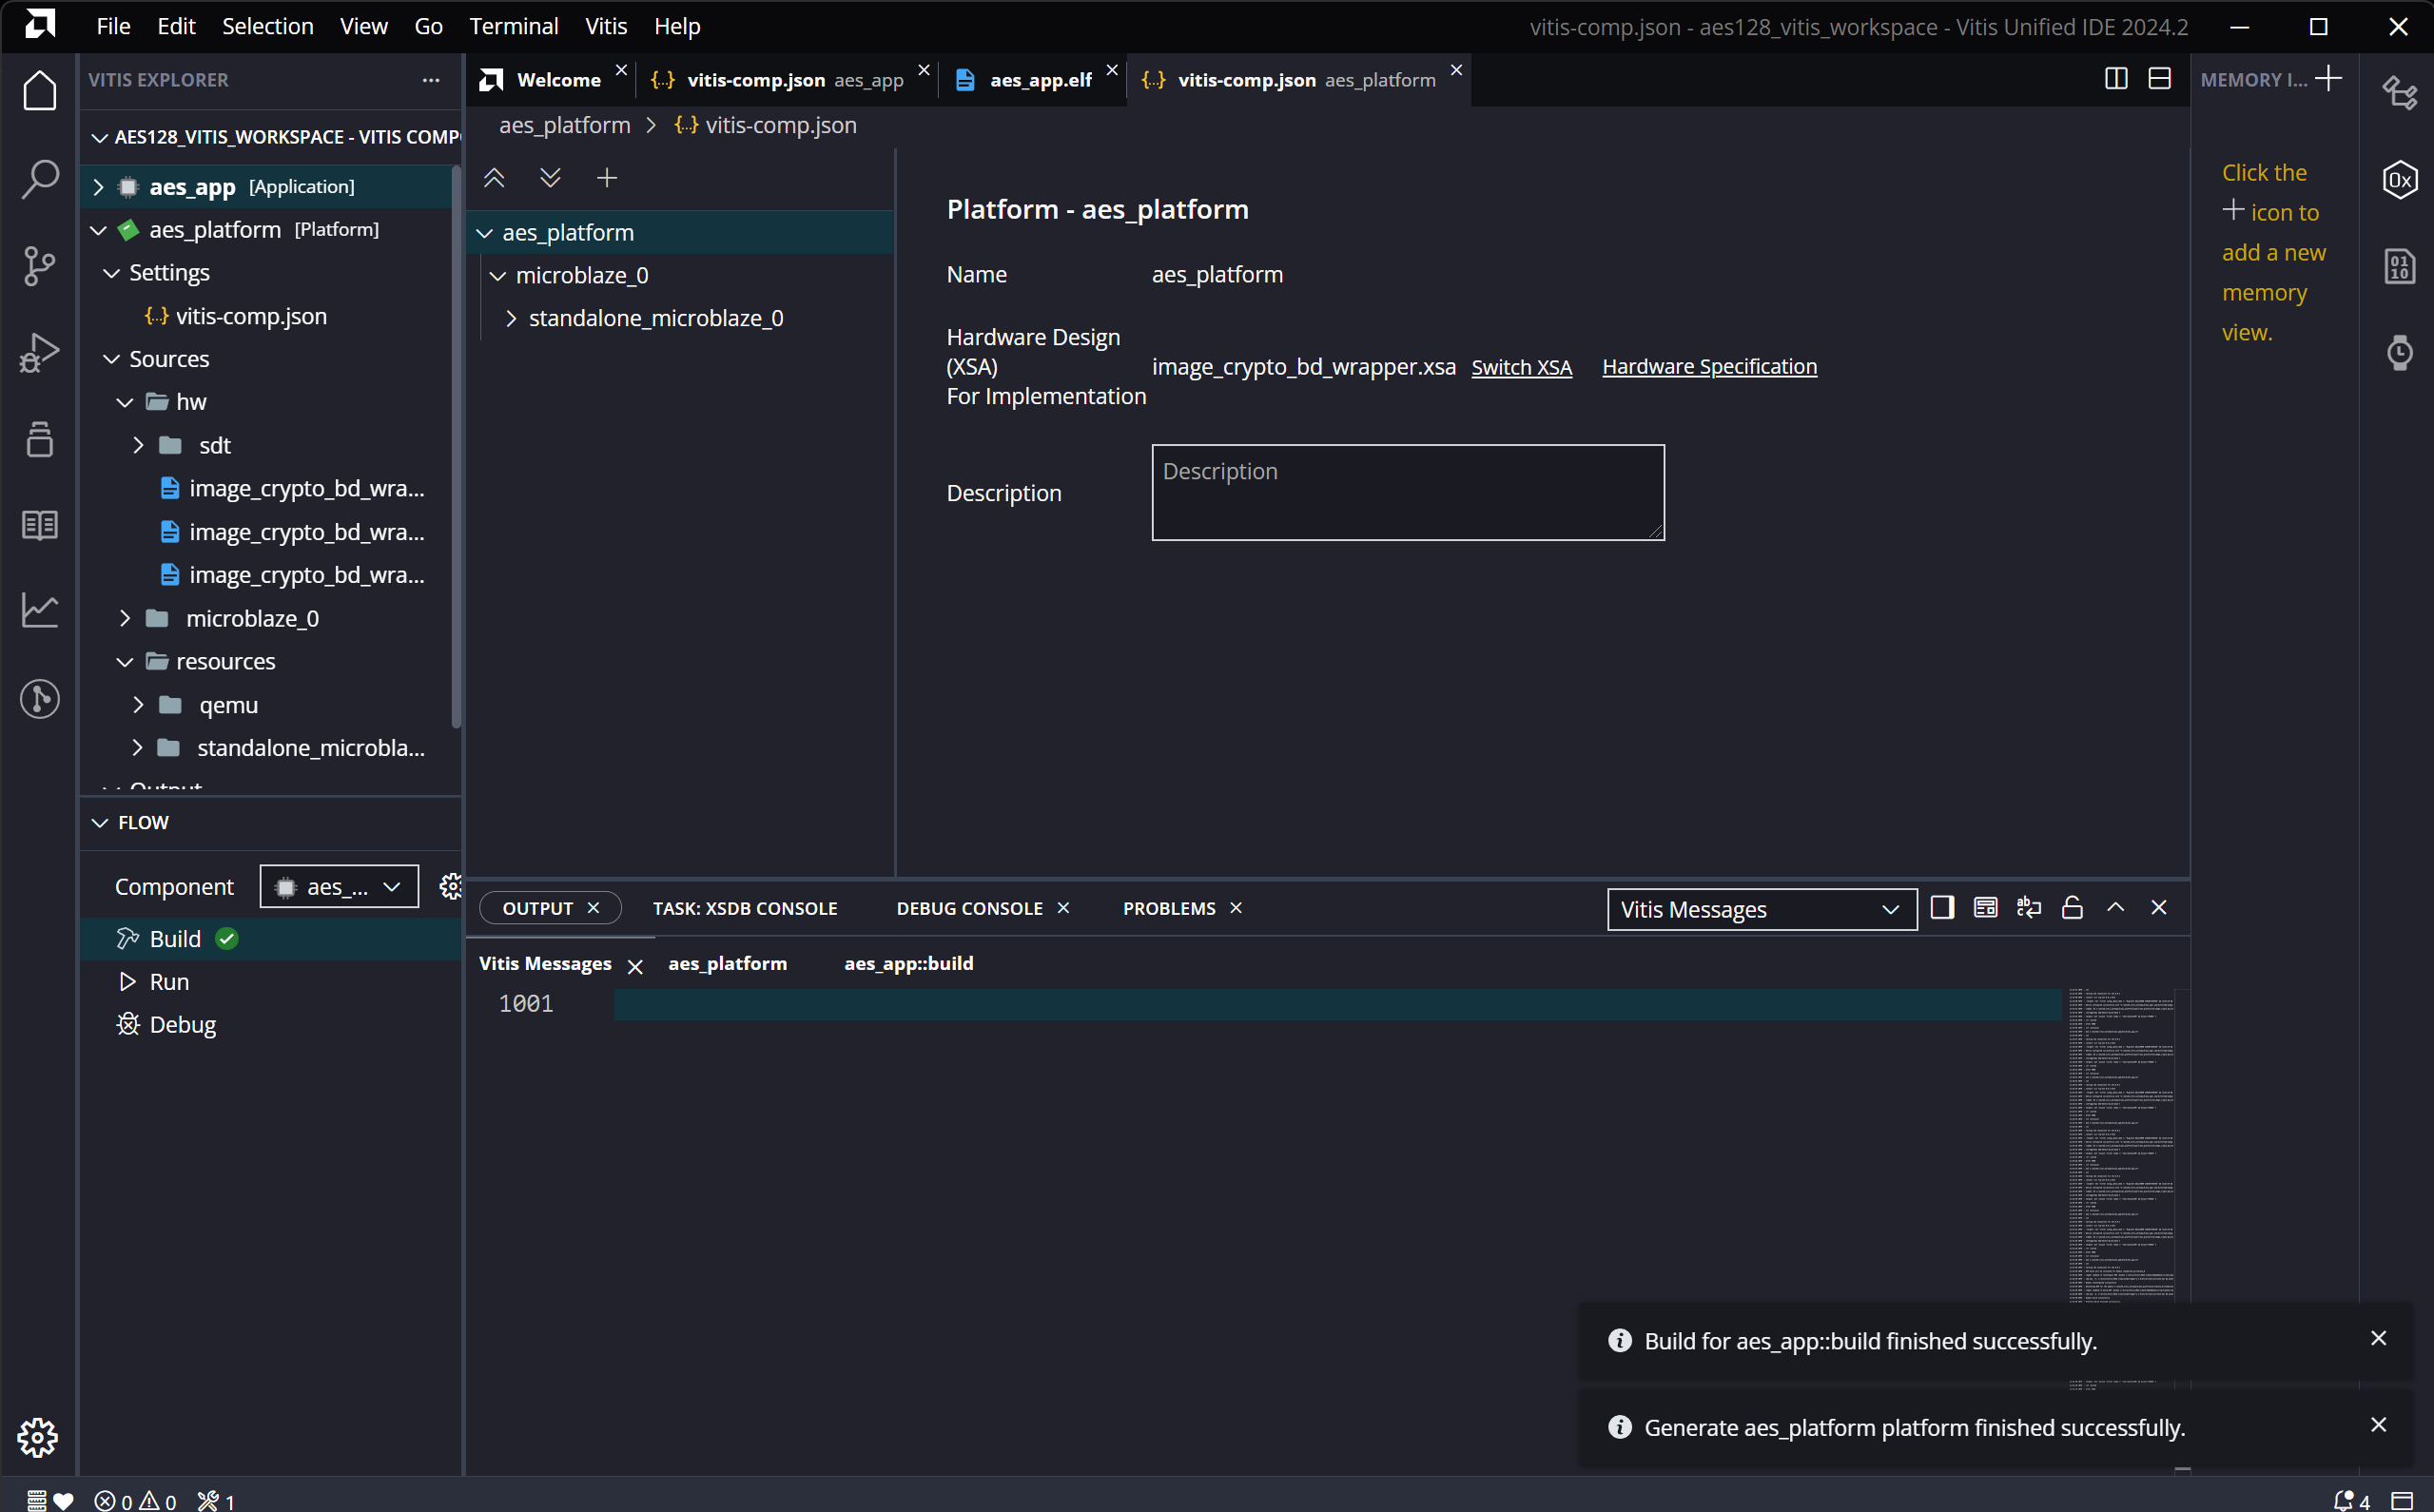
\includegraphics[width=0.85\textwidth]{vitis_project.png}
    \caption{Vitis 2024.2 IDE showing the \texttt{aes\_app} project structure with \texttt{main.c} and \texttt{aes\_ip\_driver.h}.}
    \label{fig:vitis}
\end{figure}

% ---- SECTION 5 ----
\section{Simulation and Testing}

\subsection{On-Board Testing Procedure}

Due to the UART hardware constraint (detailed in Section~\ref{sec:challenges}), all testing was performed via JTAG-based direct memory access. The complete on-board testing workflow is illustrated in Figure~\ref{fig:workflow}.

\begin{figure}[H]
\centering
\begin{tikzpicture}[
    step/.style={rectangle, draw=blue!60, fill=blue!8, rounded corners, minimum width=4cm, minimum height=0.9cm, align=center, font=\small},
    hw/.style={rectangle, draw=green!60, fill=green!8, rounded corners, minimum width=4cm, minimum height=0.9cm, align=center, font=\small},
    arrow/.style={-{Stealth[length=7pt]}, thick}
]
\node[step] (s1) at (0,0)   {1. Run AES App in Vitis\\(Programs FPGA + ELF)};
\node[step] (s2) at (0,-1.6){2. Run \texttt{auto\_dashboard.py}\\(Launches Python script)};
\node[step] (s3) at (0,-3.2){3. XSCT: Load 4096-byte\\gradient image via JTAG \texttt{mwr}};
\node[hw]   (s4) at (0,-4.8){4. User presses BTNC\\on Nexys 4 DDR board};
\node[hw]   (s5) at (0,-6.4){5. MicroBlaze: Encrypt 256\\blocks (Green LED = Done)};
\node[step] (s6) at (0,-8.0){6. User presses ENTER\\in Python terminal};
\node[step] (s7) at (0,-9.6){7. XSCT: Dump both BRAMs\\to \texttt{input\_image.raw} and \\ \texttt{output\_image.raw}};
\node[step] (s8) at (0,-11.2){8. Python: Generates HTML\\dashboard with analysis};

\foreach \a/\b in {s1/s2, s2/s3, s3/s4, s4/s5, s5/s6, s6/s7, s7/s8}
    \draw[arrow] (\a) -- (\b);
\end{tikzpicture}
\caption{Complete End-to-End Testing and Validation Workflow}
\label{fig:workflow}
\end{figure}

\subsection{Test Image Injection via JTAG}

A 64$\times$64 grayscale gradient image (4,096 bytes) was used as the test input. Since UART was bypassed, the image was injected directly into the Input BRAM at \texttt{0xC0000000} using an auto-generated Tcl script containing 1,024 individual \texttt{mwr} commands:

\begin{lstlisting}[style=tclstyle, caption={JTAG Memory Write Script (load\_explicit.tcl) Excerpt}]
connect
targets -set -filter {name =~ "MicroBlaze #0"}
mwr 0xC0000000 0xA0A0A0A0
mwr 0xC0000004 0xA0A0A0A0
...
mwr 0xC0000FFC 0xA0A0A0A0
disconnect
\end{lstlisting}

\subsection{Memory Extraction via JTAG}

After encryption (confirmed by solid Green LED), both BRAMs were read back using the \texttt{dump\_both.tcl} script which saves 4,096 bytes from each BRAM into binary raw files for analysis.

\subsection{Observed vs Expected Behaviour}

\begin{table}[H]
\centering
\caption{Simulation and Testing: Observed vs Expected Behaviour}
\begin{tabularx}{\textwidth}{lXX}
\toprule
\textbf{Test} & \textbf{Expected Behaviour} & \textbf{Observed Behaviour} \\
\midrule
LED Idle State          & LED0 (white) ON while waiting for BTNC & LED0 lit as expected \\
LED During Encryption   & LED16\_R (red) ON during 256-block loop & Red LED ON; blinks with LED0 for progress \\
LED After Encryption    & LED16\_G (green) solid ON when done & Green LED solid ON \checkmark \\
Input BRAM Content      & Gradient data (0xA0A0...) at 0xC0000000 & Verified via \texttt{mrd} readback \checkmark \\
Output BRAM Content     & Random-looking ciphertext at 0xC2000000 & Pseudo-random ciphertext verified \checkmark \\
Visual Output           & Structured image $\to$ random noise & Confirmed on dashboard \checkmark \\
Hardware Hang           & None (UART removed)                 & No hangs observed \checkmark \\
\bottomrule
\end{tabularx}
\end{table}

\subsection{Board Hardware Photos}

\begin{figure}[H]
    \centering
    \begin{subfigure}{0.48\textwidth}
        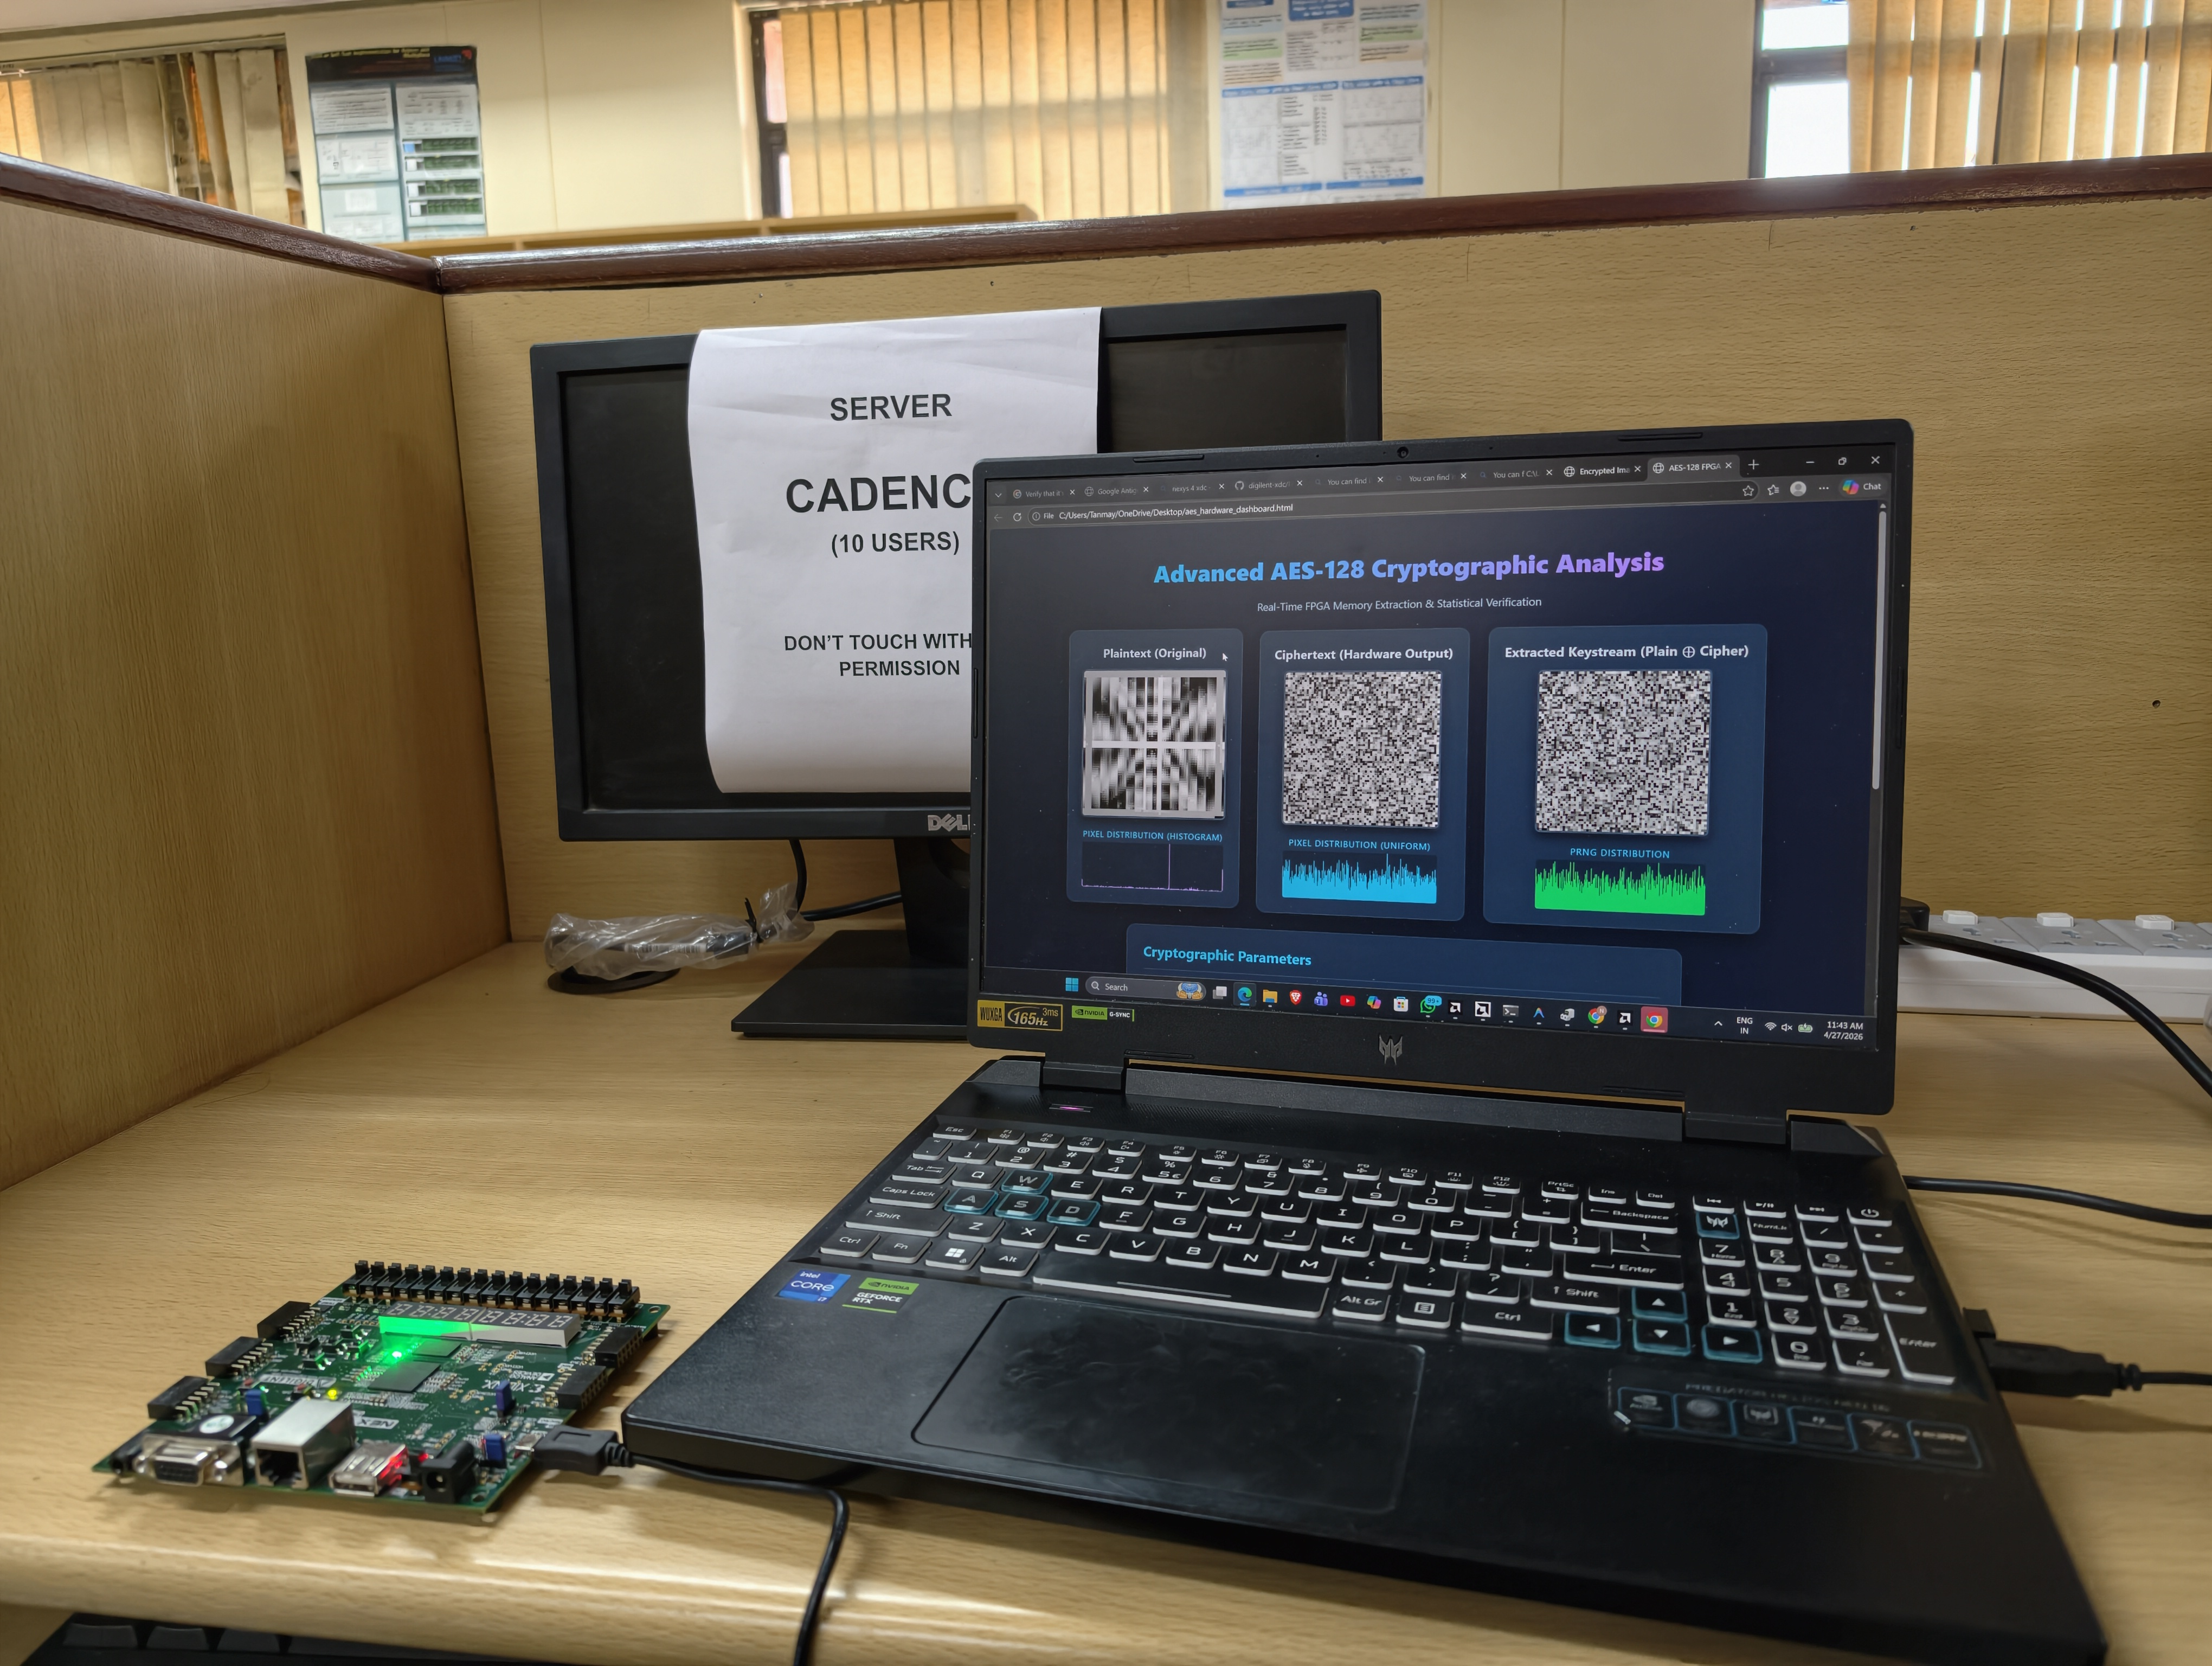
\includegraphics[width=\textwidth]{hardware_1.jpg}
        \caption{Nexys 4 DDR board powered on, green LED solid (encryption complete).}
    \end{subfigure}
    \hfill
    \begin{subfigure}{0.48\textwidth}
        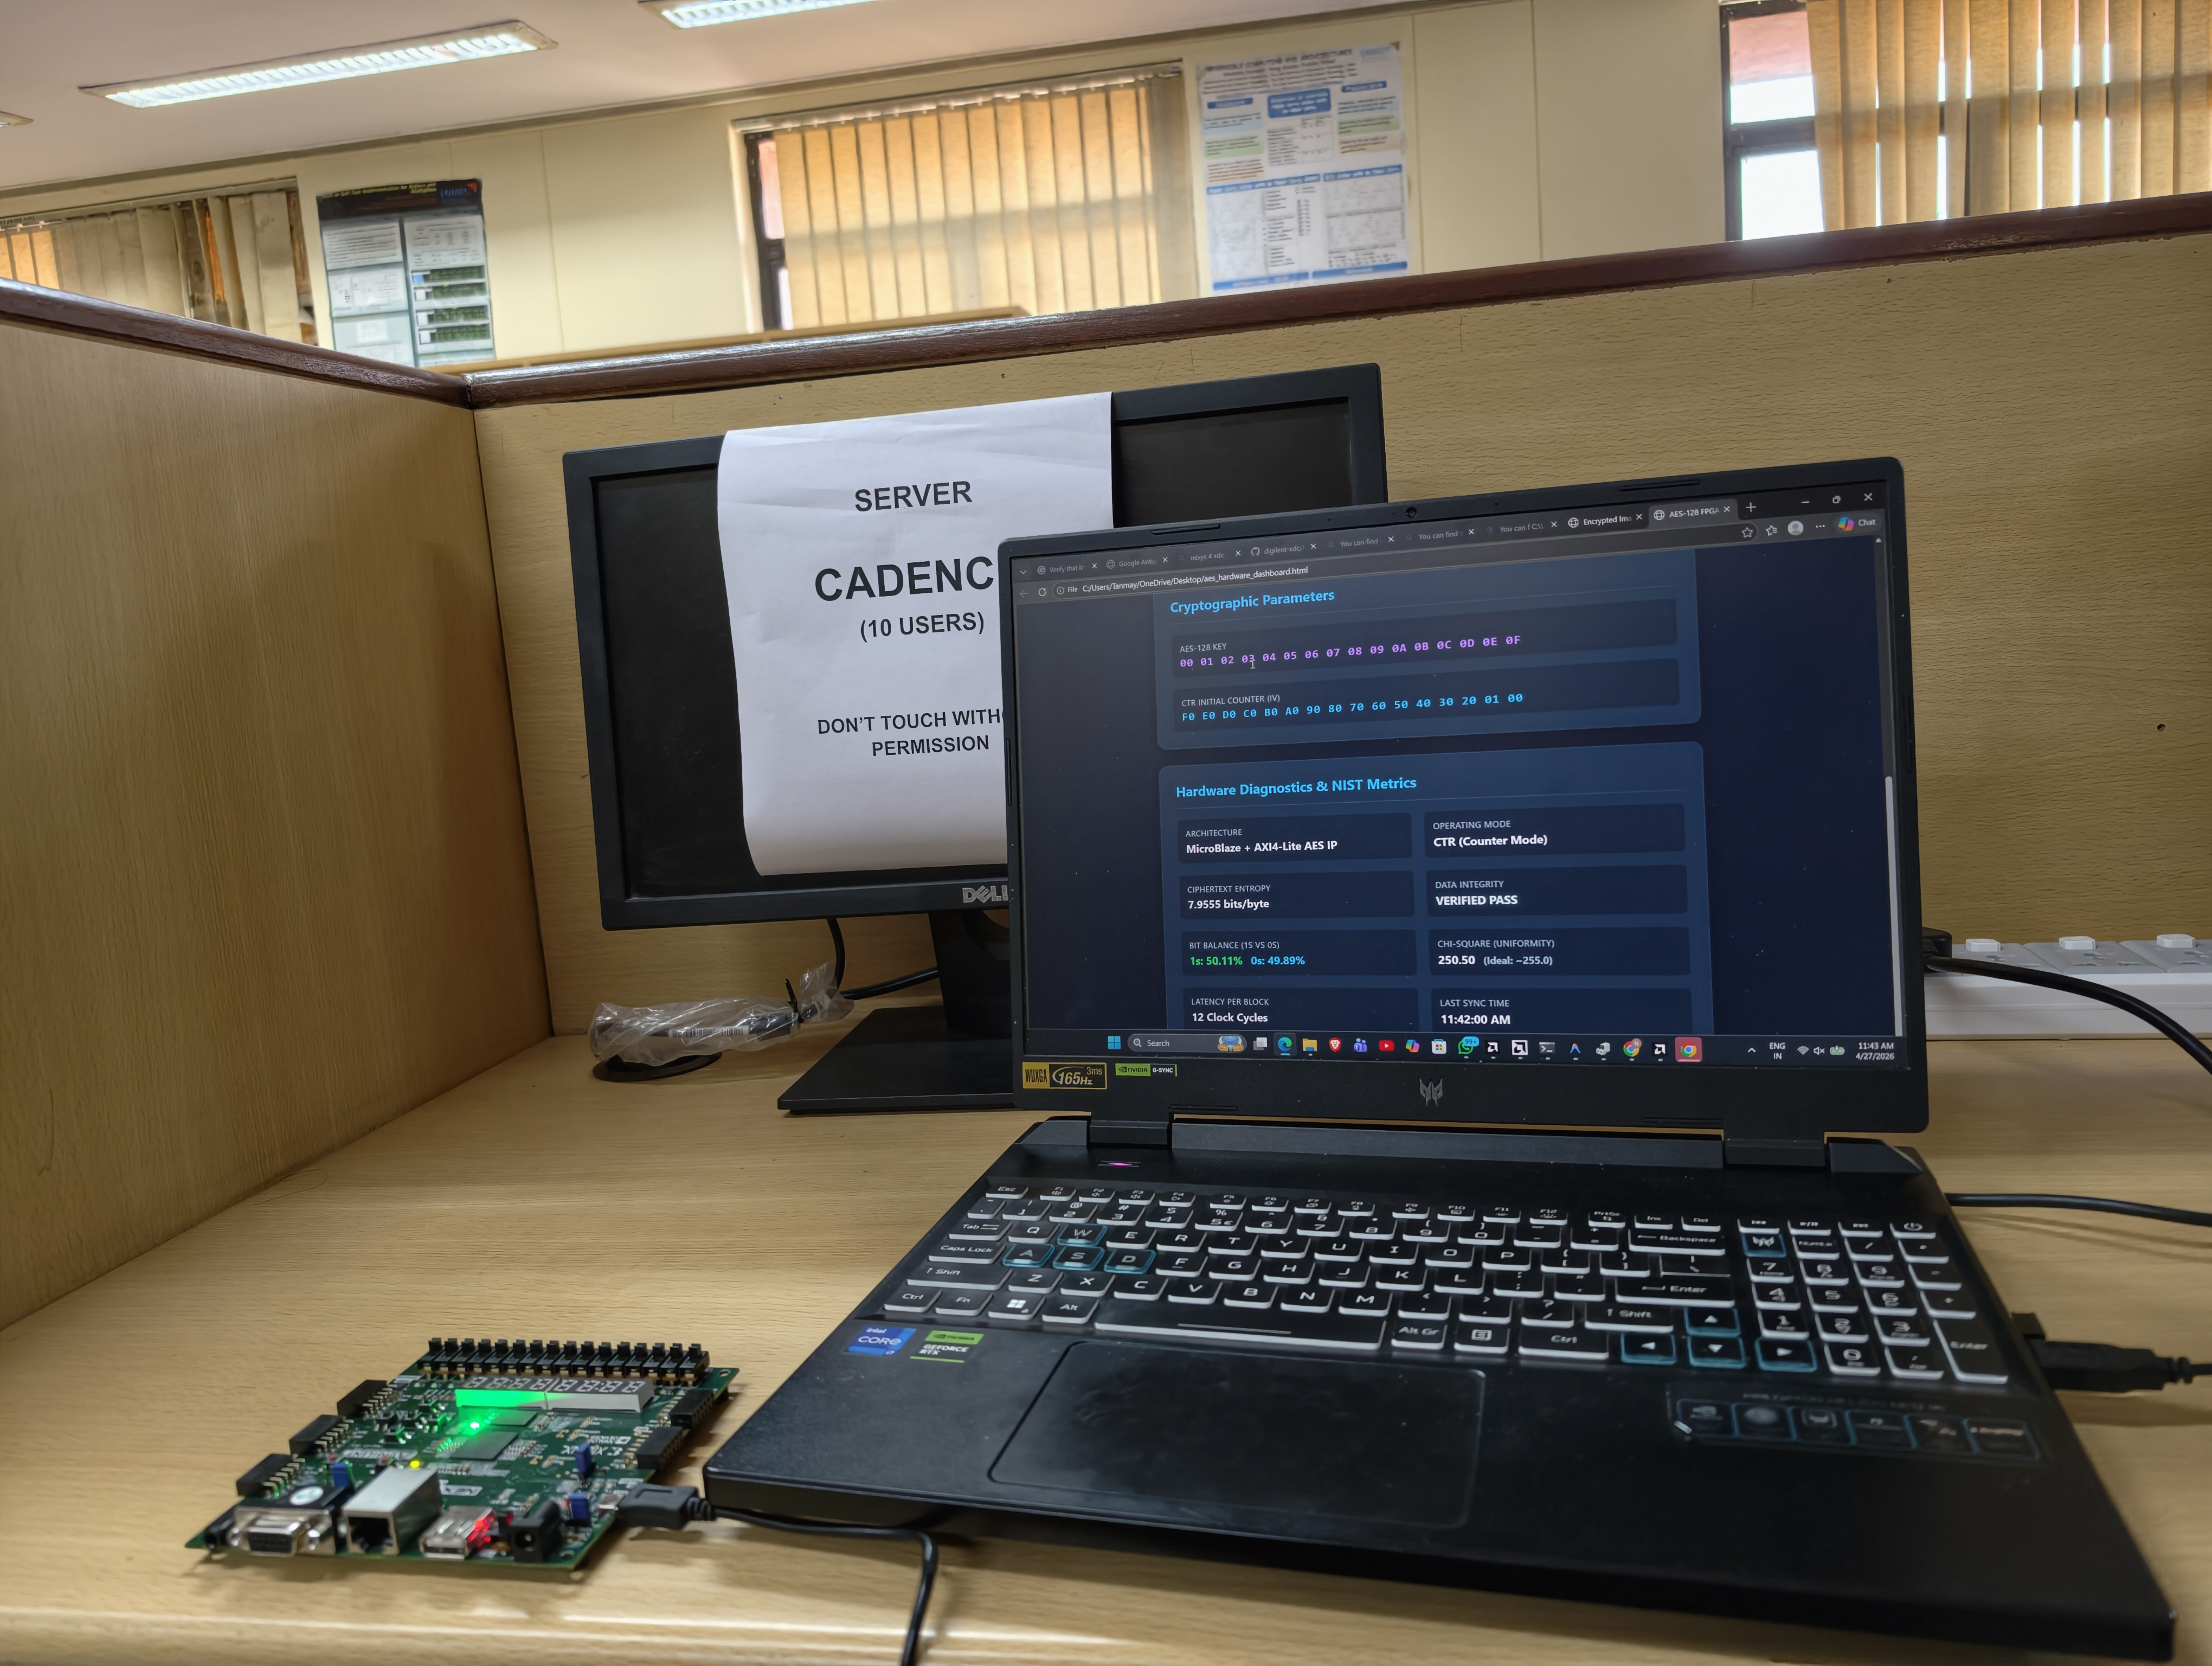
\includegraphics[width=\textwidth]{hardware_2.jpg}
        \caption{Board during active operation.}
    \end{subfigure}
    \caption{Live Hardware Validation on Nexys 4 DDR FPGA Board}
    \label{fig:board_photos}
\end{figure}

\subsection{Python Terminal Screenshot}

\begin{figure}[H]
    \centering
    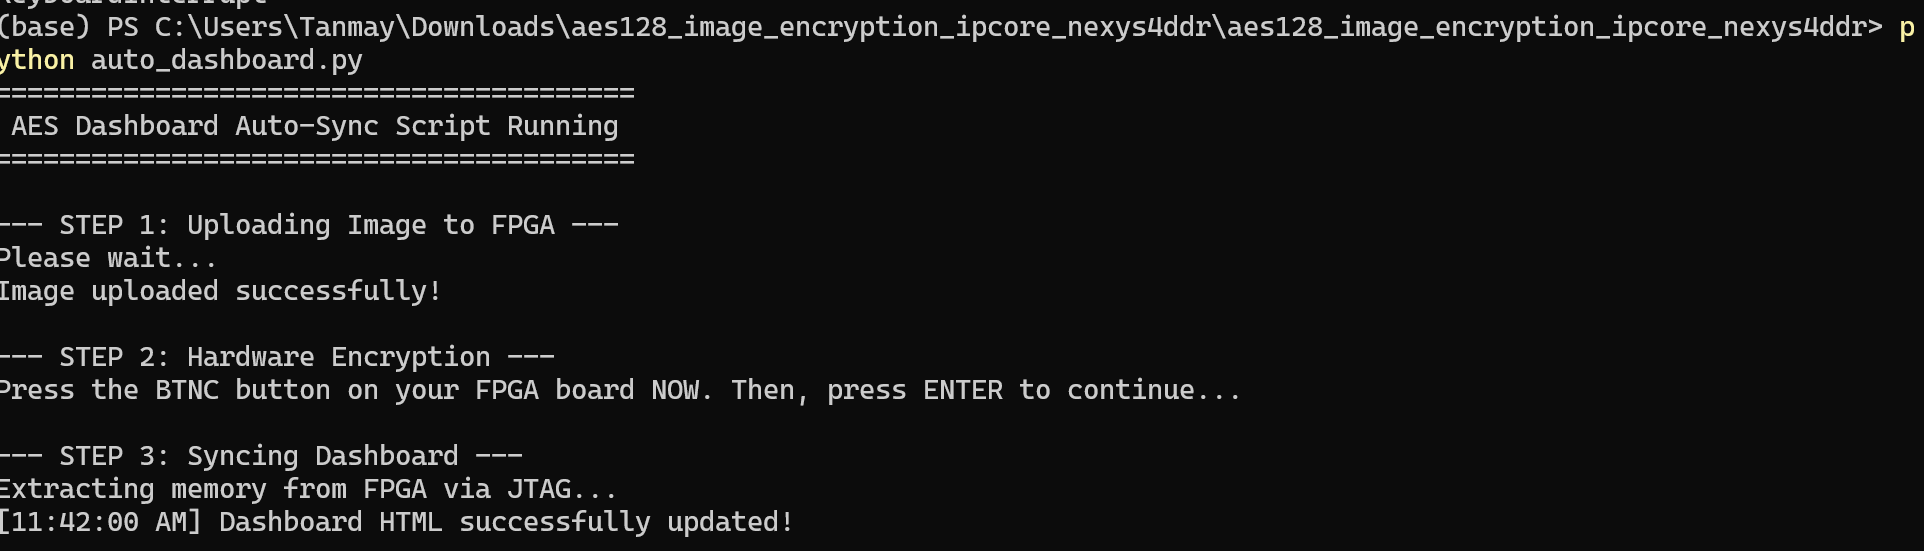
\includegraphics[width=0.9\textwidth]{python_terminal.png}
    \caption{Terminal output of \texttt{auto\_dashboard.py} showing all 3 steps: image upload, encryption trigger, and dashboard sync.}
    \label{fig:python_term}
\end{figure}
